\chapter{The SPACE Analysis}
After introducing the detector workings, reconstruction and analysis techniques, background contributions and the signature of the signal, this chapter gives an overview of analysis. Starting from data processed with basic reconstructions and requirements a workflow was set up to try to discriminate events that are most likely of known physical interactions from the rare events that are sought for in this analysis. These events would originate from the theoretical particles with an anomalous charge (see Chapter \ref{ch:theoreticalmotivation}). The analysis was adopted the "SPACE" analysis, which stands for a "Search for Particle with Anomalous ChargE".

\section{Filter selection}
As explained in Section \ref{subsec:filters}, the data is processed through multiple filters. Since this analysis is the first of its kind in the collaboration, no processed dataset from other analyses was used. Filters had to be selected for proper comparison of data and Monte Carlo and I have chosen to optimize the signal to background ratio to select which filters should be included. An illustration is given in Fig. \ref{fig:filterrate}. This filter selection will be referred to as \textit{Level2b}, as a simple addition to filter processing in Level2 (see Section \ref{sec:processing}). 

\begin{figure}
\centering
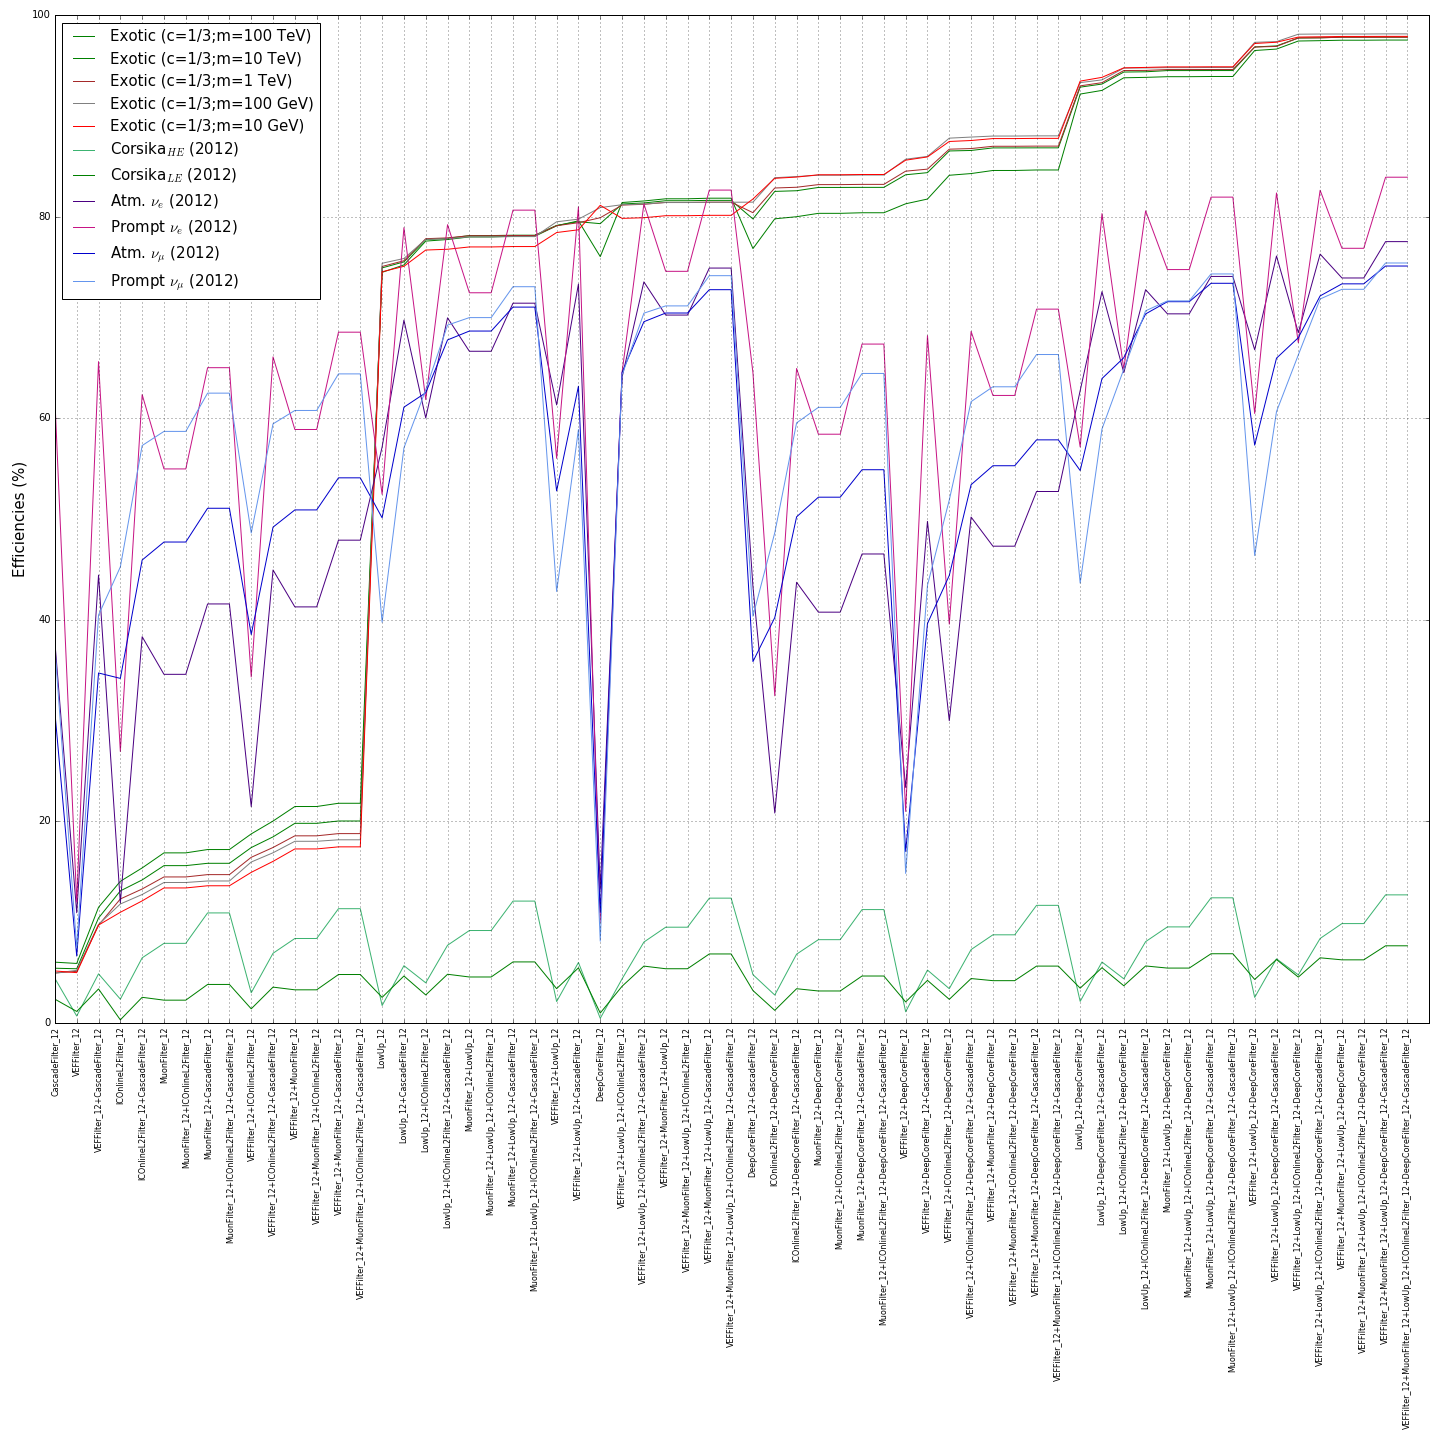
\includegraphics[width=\textwidth]{chapter8/img/FilterRate.png}
\caption{Illustration of the efficiencies of several filters and their possible combinations. The x-axis was determined by starting with filter selections that had a low efficiency in signal selection and range in function of performance. Five signal points for a fixed charge and different mass show similar results. Exotic SMPs with charges 1/2 and 2/3 show very similar results but are left out for a better visualization.}
\label{fig:filterrate}
\end{figure}

\subsection{VEF}
The Vertical Event Filter (VEF) is designed to be used for oscillation and Earth WIMP analyses and makes use of the string trigger (see Section \ref{subsec:triggers}). An SMP that travel alongside a string, or closeby, can trigger optical modules while the total light yield of an event is low, making this filter an ideal addition to the filters that are selected. In addition, the filter removes HLC hits in the top 5 DOM layers to reduce the muonic component from air shower events. Other selection cuts, try to optimize the search efficiency for WIMP events in particular. For example, the LF zenith angle should be higher than 68.7$^\circ$. More information can be found in Ref. \cite{VEF2012}.

%meeste hiervan: https://docushare.icecube.wisc.edu/dsweb/Get/Document-62750/VEF_2013_proposal.pdf

\subsection{LowUp}
The LowUp filter is again mainly designed for WIMP searches, but also atmospheric neutrino analysis and is mainly designed to capture up-going muons with an energy below 1 TeV. The majority of the events that are selected by this filter make use of the in-ice Volume Trigger (see Table \ref{tab:trigger}), but also the in-ice SMT8, in-ice String and SMT3-DeepCore triggers are run over for completeness. The selection cuts are loose selections required to look for up-going track-like particles. For example, the zenith angle of the reconstructed particle should have an angle of 80$^\circ$ or higher and the difference between the maximal z-coordinate and minimal z-coordinate of hit DOMs should be less than or equal to 600 m. More information can be found in Ref. \cite{LowUp2012}.

%je hebt een Nchan>=5 cut in je L4 zodat veranderingen in LowUp niet uitmaken :-)

\subsection{Online Muon L2}
The Online Muon L2 filter is a subset of the Muon Filter (see Ref. \ref{Muon2012}) and tries to select the most interesting muon-like events while reducing the rate of the filter from around 30 Hz to 5 Hz, reducing the data with a factor of 6. Historically this subset was processed data from the Muon Filter, but after realizing that this could be done online and because many analyses made use of this selection, it was chosen to implement it as a separate filter. The filter tries to select both up-going and down-going muons, with different selection cuts depending on the zenith angle of the particle reconstruction. The four selection ranges are defined as:
\vspace{2mm}
\begin{itemize}
\item $180^\circ \geq \theta_\textrm{MPE} \geq 115^\circ$
\item $115^\circ > \theta_\textrm{MPE} \geq 82^\circ$
\item $82^\circ > \theta_\textrm{MPE} \geq 66^\circ$
\item $66^\circ > \theta_\textrm{MPE} \geq 0^\circ$
\end{itemize}
where the particle reconstruction was done with MPE (Section \ref{subsec:spempe}), which was feasible if it only had to be done on the events passing the Muon Filter. The first two regions have an efficiency\footnote{Here defined as having a reconstruction within 3$^\circ$ of the MC truth.} higher than 99\%. The down-going region require more stringent cuts to remove the less interesting muons from air showers. The variables used are the number ot hit DOMs, likelihood parameters, number of PEs and so on. More information can be found in Ref. \cite{OnlineMuonL22012}.

\textcolor{red}{Verhoogt uw signaal niet zo veel omdat je enkel upgoing signaal gebruikte om dit te testen.}

\subsection{DeepCore}
Additionally a DeepCore specialized filter was added to account for SMP tracks that partially traverse the more densly instrumented DC detector. Due to the low amount of light produced by these dim tracks, adding the DeepCore filter that is specialized for this part of the detector proved to be of significant importance.

The DeepCore filter was designed to look for very dim events coming from, e.g., dark matter, low-energy neutrino oscillations, and studies in observing atmospheric neutrinos below 100 GeV. The fiducial volume used for this filter consists of
\vspace{2mm}
\begin{itemize}
\item the bottom 22 DOMs on the IceCube strings 25, 26, 27, 34, 35, 36, 37, 44, 45, 46, 47 and 54;
\item the bottom 50 DOMs on the DeepCore strings 79-86.
\end{itemize}
\vspace{2mm}
These strings are indicated in Fig. \ref{fig:deepcorestrings}.\\

\begin{figure}[t]
\centering
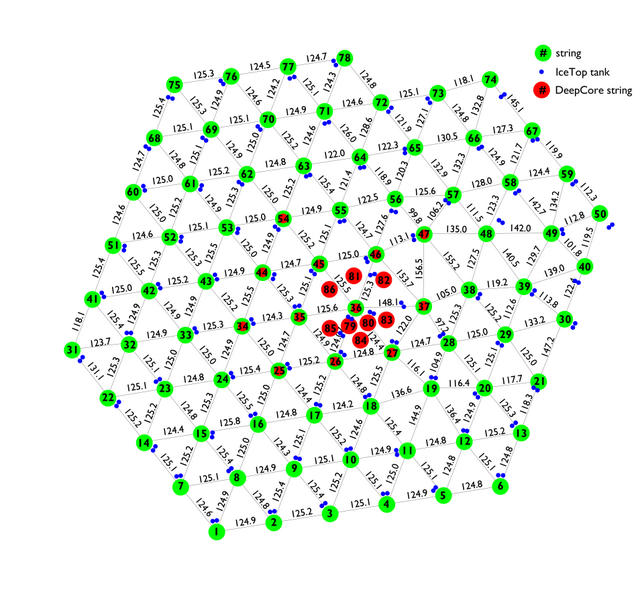
\includegraphics[width=0.55\textwidth]{chapter8/img/stringview.jpg}
\caption{Aerial view of the IceCube strings (and IceTop tanks) where the DeepCore fiducial volume is defined by the DeepCore strings (red) and several surrounding in-ice IceCube strings (green and red).}
\label{fig:deepcorestrings}
\end{figure}

\noindent The filter uses the DeepCore SMT3 trigger and calculates the COG position. Two layers are used as a veto to remove events that probably originate from atmospheric muons. More information can be found in Ref. \cite{DeepCore2012}.

\subsection{Burnsample checks}
Before further processing, the burn sample (Section \ref{sec:burnsample}) is compared over the different years that are used in the analysis. This is shown in Figure \ref{fig:burnsamplechecks}. More information on the burn sample can be found in Section \ref{sec:burnsample}.

\begin{figure}[t]
\centering
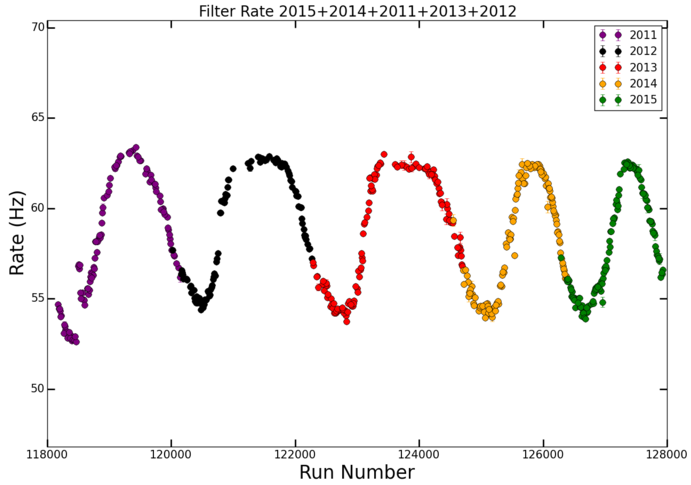
\includegraphics[width=0.49\textwidth]{chapter8/img/FilterRatePerRun.png}
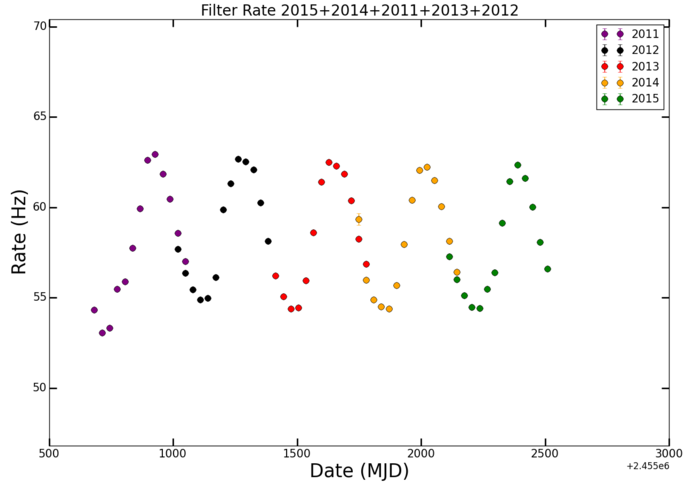
\includegraphics[width=0.49\textwidth]{chapter8/img/FilterRatePerMonth.png}
\caption{\textit{Left: }Total rate of the combined filters in function of the run number. The sine wave pattern from seasonal variations in the atmosphere (see Section \ref{subsub:corsika}) is clearly visible and consisten throughout the years. The x-axis is more spread out in the first years as there were more test runs. The shift in data rate in early 2011 runs is due to the DOM software change that was introduced in the Summer of 2011 \cite{2011rate}. This phenomenon is well understood and since the changes are minimal it was chosen to keep these runs. \textit{Right: }Total filter rate averaged per month. There is an overlap for each year because a new season doesn't necessarily start in the beginning of a month.}
\label{fig:burnsamplechecks}
\end{figure}

\section{Quality cuts}
The combined filter selection leads to a total rate of $\sim60$ Hz, or $\sim1.9$ billion events per year. 
MPE 



De uitleg van temperature modulations is goed in Sam zijn thesis
\url{https://arxiv.org/pdf/physics/0312102v1.pdf}\\
\url{https://arxiv.org/pdf/1310.1284.pdf}

Ook ergens een tabel maken met info over je data runs. Duidelijk maken wat de livetime is bv en ook zeggen van wanneer to wanneer een bepaalde run liep (2011: mei 2011- mei 2012)

Klaus zijn paper? \url{https://arxiv.org/abs/1806.05696}

\section{Motivation}
\section{General strategy}
\section{Event cleaning}
\section{Variables}
\section{BDT results}
\section{Pull validation}
\section{Systematic Uncertainties}

\section{Results}